\begin{Huge}
	Informatik (Bachelor of Education)-FAQ
\end{Huge}
\begin{block}{Häufig gestellte Fragen zum Studium}
\begin{large}
	\begin{itemize}
		\item \textbf{Lernt man im Studium, wie man programmiert?}
\begin{itemize}
	\item Ja, aber auf einer sehr eigenständigen Basis. Man bekommt eine Überblick über die Sprache(n), alles andere was darüber hinaus geht muss man sich selbst aneignen.
\end{itemize}

\item \textbf{Welche Programmiersprachen macht man da so?}
\begin{itemize}
	\item Ist vom Professor abhängig. In den ersten beiden Semestern meistens entweder Java oder Racket, manchmal auch C++.
\end{itemize}

\item \textbf{Muss man programmieren können, um das Studium anzufangen?}
\begin{itemize}
	\item Nein. Die Vorlesung beginnt absolut bei 0, um allen den Einstieg zu ermöglichen.
\end{itemize}


\item \textbf{Muss man gut in Mathe sein?}
\begin{itemize}
	\item Man muss kein Mathe-Genie sein, man sollte Mathe aber nicht hassen. Auch wenn man nur Mathe I hat, benötigt man für die Informatik einiges an mathematischer Denkweise.
\end{itemize}
\item \textbf{Welche Fächer kann man mit Informatik kombinieren?}
\begin{itemize}
	\item Alles außer NWT.
\end{itemize}
\item \textbf{Was, wenn ich merke, dass Lehramt doch nichts für mich ist?} 
\begin{itemize}
	\item Du kannst Informatik gegen ein anderes Fach tauschen oder dich vom B.Ed. verabschieden und auf ein "`normales"' B.Sc.-Studium wechseln.
\end{itemize}
\item \textbf{Was mache ich denn mit einem Bachelor of Education?} 
\begin{itemize}
	\item Die kurze Antwort: Weiter machen. Der Bachelor ist nur ein Teil deines Lehramtsstudiums, danach folgen noch der Master und das Referendariat.
\end{itemize}
\item \textbf{Wie sind meine Berufsschancen?} 
\begin{itemize}
	\item Da in BaWü ein großer Informatiklehrermangel herrscht, sind deine Berufschancen sehr hoch.
\end{itemize}
\item \textbf{Was ist denn der Unterschied zwischen B.Sc. und B.Ed?} 
\begin{itemize}
	\item Im B.Ed. hört man ein paar weniger Informatikvorlesungen als im B.Sc. und hat dafür Vorlesungen zu Bildungswissenschaften und Fachdidaktik.
\end{itemize}
\item \textbf{Was ist Fachdidaktik?} 
\begin{itemize}
	\item In Fachdidaktik lernt man, wie man sein Wissen SuS~ (Schülerinnen und Schülern) beibringt und wie man Unterricht am besten planen kann.
\end{itemize}

\item \textbf{Gibt es Praktika?}
\begin{itemize}
	\item Ja, nachdem du BWS-I bestanden hast, musst du ein dreiwöchiges Orientierungspraktikum an der Schule machen, das in den Semesterferien stattfindet. Man hat zum Ablegen dieses Praktikums aber bis zum Ende des Bachelors Zeit. Im Master gibt es dann noch ein komplettes Semester Schulpraxis.
\end{itemize}

\item \textbf{Wie ist da so der NC?}
\begin{itemize}
	\item Gibt es keinen.
\end{itemize}
\item \textbf{In welchen Klassenstufen wird Informatik unterrichtet?}
\begin{itemize}
	\item Hier ein kleines Schaubild zur Erläuterung, wie es eigentlich sein sollte:
	\begin{figure}[h!]
	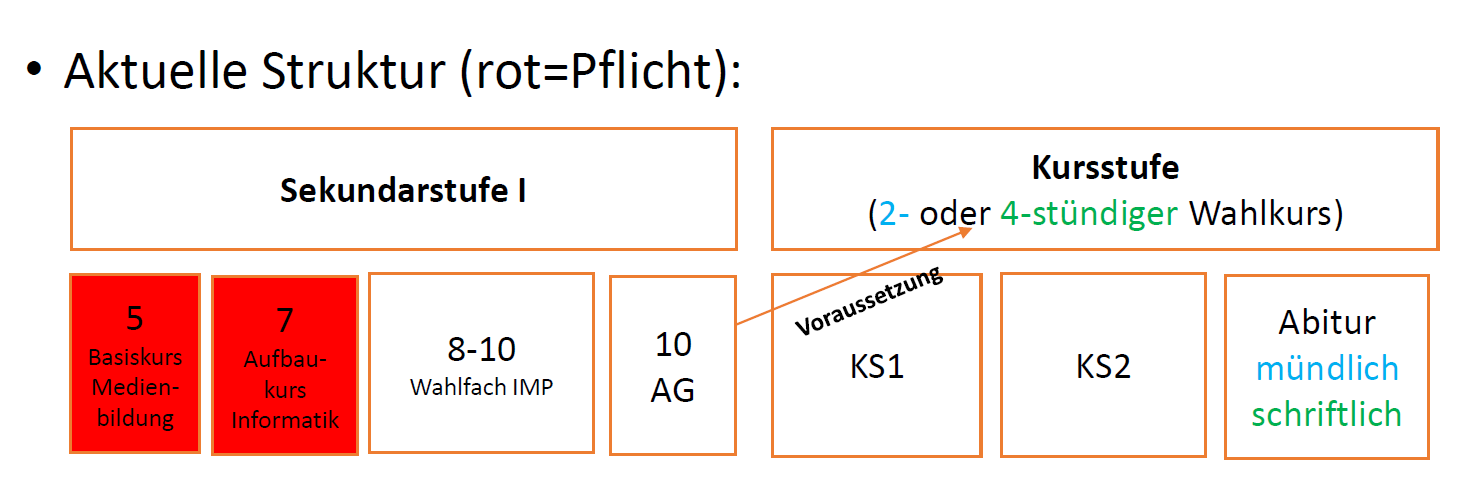
\includegraphics[width=0.6\linewidth]{charts/info_bed_klassenstufen.png}
	\end{figure}
	Momentan ist es aber leider so, dass sich Schulen aufgrund des Lehrermangels kaum an diesen Lehrplan halten können.
\end{itemize}
	\end{itemize}
\end{large}
\end{block}
